\section{Results}\label{sec:results}
We quantify the Jao Gap location along the magnitude axis by sub-sampling our
synthetic populations, finding the linear number density along the magnitude
axis of each sub-sample, averaging these linear number densities, and
extracting any peaks above a prominence threshold of 0.1 as potential
magnitudes of the Jao Gap. Figure \ref{fig:JaoGapLocator} shows this fit for
both OPAL and OPLIB populations.

\begin{table}
	\centering
	\begin{tabular}{c | c c}
		\hline
		Model & Location & Prominence \\
		\hline
		\hline
		OPAL & 10.15864 & 0.19501 \\
		OPLIB 1 & 10.17813 & 0.26055 \\
		OPLIB 2 & 10.21313 & 0.46898
	\end{tabular}
	\caption{Locations identified as potential Gaps.}
	\label{tab:GapLocation}
\end{table}

Our Gap identification method finds two potential Gaps in the OPLIB (Table
\ref{tab:GapLocation}) data while only finding one in the OPAL dataset. This
apparent discrepancy is not due to a fundamental structural difference between
the OPAL and OPLIB opacity tables; rather, it is attributable to the
phasing of the periodic luminosity variations seen across mass in Figure
\ref{fig:PunchIn} and whether or not the
injected noise smears all of these together into one Gap or two Gaps.

{\color{red} [There will be text detailing a test where I manually shift the
OPAL data to the same phase as the OPLIB in an attempt to explain the extra Gap
seen in OPLIB]}.

\begin{figure}
	\centering
	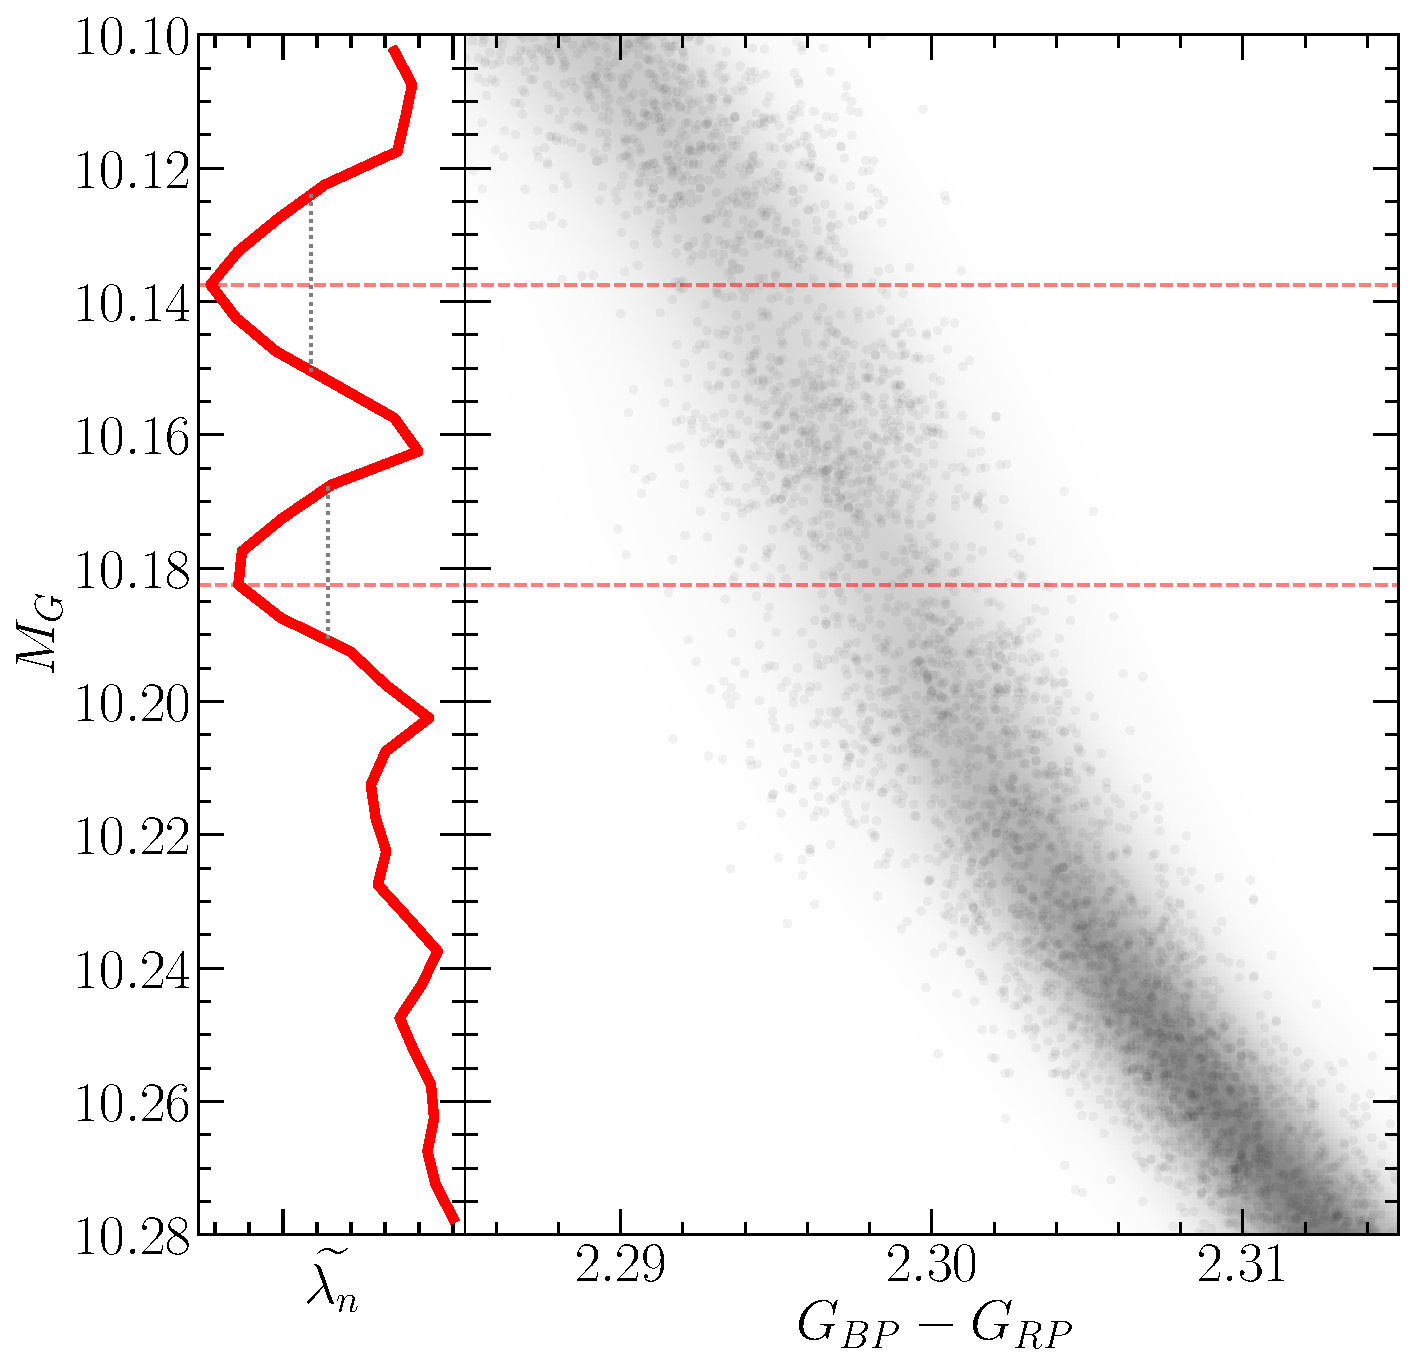
\includegraphics[width=0.45\textwidth]{src/figures/NotebookFigs/OPAL_Jao_locator.png}
	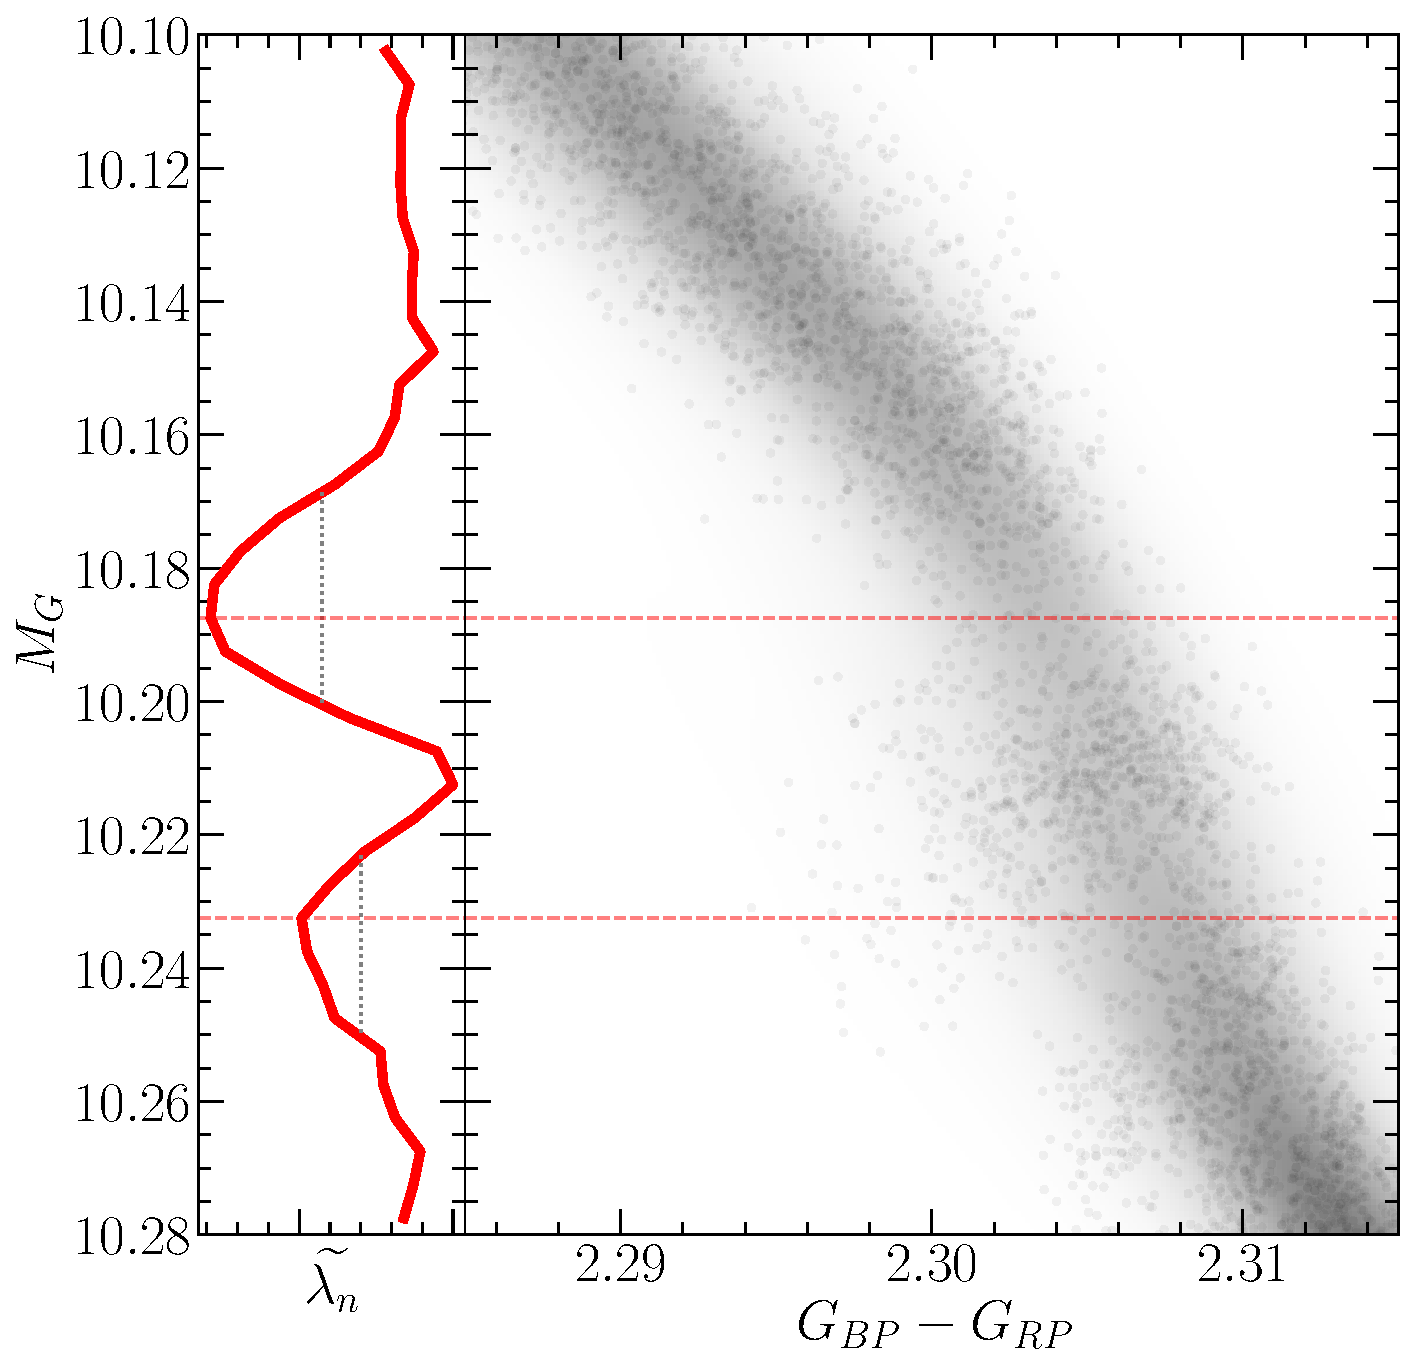
\includegraphics[width=0.45\textwidth]{src/figures/NotebookFigs/OPLIB_Jao_locator.png}
	\caption{(right panels) OPAL (top) and OPLIB (bottom) synthetic
	populations. (left panels) Normalized linear number density along the
	magnitude axis. A dashed line has been extended from the peak through both
	panels to make clear where the identified Jao Gap location is wrt. to the
	population. }
	\label{fig:JaoGapLocator}
\end{figure}

Both Gaps identified in the OPLIB sample are at fainter magnitudes than the Gap
identified in the OPAL sample. Consequently, in the OPLIB sample the
convective mixing events which drive the kissing instability happen more
regularly and therefore also start earlier in the model's evolution. This is
because each mixing event serves to interrupt the ``standard'' luminosity
evolution of a stellar model, kicking its luminosity back down to what it would
have been at some earlier stage of stellar evolution instead of allowing it
to slowly increase.
% Looking at the interior physics of one OPAL and one OPLIB
% model shows that this shorter duration between mixing events (Figure
% \ref{fig:OPALOPLIB3He}).

Convective mixing events starting earlier in a model's evolution are consistent
with the slightly lower opacities characteristic to OPLIB. A lower opacity
fluid will have a more shallow radiative temperature gradient than a higher
opacity fluid; however, as the adiabatic temperature gradient remains
essentially unchanged as a function of radius, a larger interior radius of the
model will remain unstable to convection {\color{red}[CHECK IF THIS OR IF
RADIATIVE ZONE MOVING IN]}. This larger convective zone, and therefore smaller
radiative zone, is in line with the behavior of the models presented here as it
with the radiative zone closer to the convective zone it takes less time for
that radiative zone to heat up and become unstable to convection. We see that
OPLIB models undergo convective mixing events earlier in their evolution than
OPAL models (Figure \ref{fig:OPALOPLIB3He}) implying that the inner convective
zone did not have to expand as much to meet the outer convective zone. 

\begin{figure}
	\centering
	\includegraphics[width=0.45\textwidth]{src/figures/NotebookFigs/3HeOPAL_OPLIB.pdf}
	\caption{Core $^{3}$He mass fraction for a model evolved with OPAL and a
	model evolved with OPLIB within the Jao Gap's mass range. Note how the
	OPLIB model undergoes the mixing event earlier in its evolution than the
	OPAL model does.}
	\label{fig:OPALOPLIB3He}
\end{figure}

The most precise published Gap location comes from \citet{Jao2020} who use EDR3
to locate the Gap at $M_{G} \sim 10.3$, we identify the Gap at a similar
location in the GCNS data. \textbf{The Gap in populations evolved using OPLIB tables
is closer to this measurement than it is in populations evolved using OPAL tables
(Table \ref{tab:GapLocation}).} It should be noted that the exact location of
the observed Gap is poorly captured by a single value as the Gap visibly
compresses across the width of the main-sequence, wider on the blue edge and
narrower on the red edge such that the observed Gap has downward facing a wedge
shape (Figure \ref{fig:JaoGap}). This wedge shape is not successfully
reproduced by either any current models or the modeling we preform here. We
elect then to specify the Gap location where this wedge is at its narrowest, on
the red edge of the main sequence.

The Gaps identified in our modeling have widths of approximately 0.03
magnitudes, while the shift from OPAL to OPLIB opacities is anywhere from 0.02
to 0.05 magnitudes. With the prior that the Gaps clearly shift before noise is
injected we know that this shift is real. However, since the shift magnitude
and Gap width are of approximately the same size in our synthetic populations
its likely that in a real population --- with both compositional and age
variations which we do not account for --- \textbf{the Gap location will not
provide a usable constraint on the opacity source.}
